\subsection{Tests}
\FuncReq
\graphicspath{ {images/} }

{Running Apache Flink with defined data sink}
{For this test I ran Apache Flink code that I got from the Gladios Data team's repository.The system's defined data sink is \textbf{\textit{  text.map(new Mapper()).writeAsText("C:/Users/rob/Documents/NetBeansProjects/COS301/test.txt");}} but this line will only work on one computer and did not run when we tested it. As can be seen in \textbf{Figure 1}, the reason why the file directory cannot be found is because it is only specified for one computer.
			\begin{figure}[h]
				\centering
				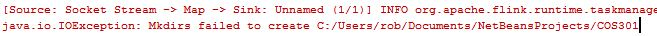
\includegraphics{wrong_file_error.jpg}
				\caption{Wrong File Path}
				\label{fig:WrongFIlePath}
			\end{figure} }
{Critical}
{0}
{Fail}
		

{Running Flink after changing data sink}
{For this test I ran Apache Flink code but I changed the data sink to \textbf{\textit{  text.map(new Mapper()).writeAsText(/"tmp/test.txt");}}, so that the system can run on any computer. After changing the data source the system runs without any error and returns a devices location in the text file, as can be seen in \textbf{Figure 2}.As a side note is shows that the result is the Longitude and Latitude but it is actually the x and y values relative to the access point.
		\begin{figure}[h]
			\centering
			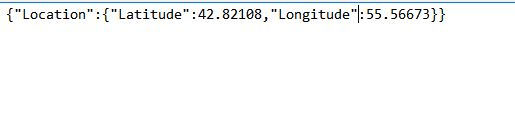
\includegraphics{query_location_results.jpg}
			\caption{Output}
			\label{fig:Output}
		\end{figure} 
}
		
{N/A}
{8}
{Pass}
		
{Running flink without starting the Job Manager}
{This test will see if Apache Flink runs and returns the relevant information without starting the Job Manager. Flink does run without a Job Manager and returns the same result which can be seen in Figure 2 of the previous test.}
{N/A}
{10}
{Pass}

{Does the current system stream data}
{Currently Gladios Data only queried a devices mac address once. From this test the system return a devices location, which can be seen in \textbf{Figure 3}.
		\begin{figure}[h]
			\centering
			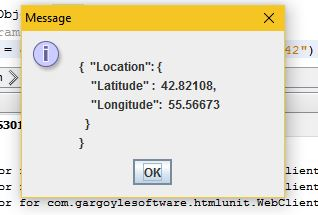
\includegraphics{right_mac.jpg}
			\caption{Correct Mac Address}
			\label{fig:right_mac}
		\end{figure} 
}
{N/A}
{9}	
{Pass}	
	
{Can the system stream and handle 2000 requests} 
{For this test case a for loop is used and queries 2 mac addresses 1000 times. The code can be seen in Figure 4. The system only returns the location of one mac address and does not do anything after that. From this I, can conclude that the Gladios Data module cannot take a data stream in nor produce an output data stream.
	\begin{figure}[h]
		\centering
		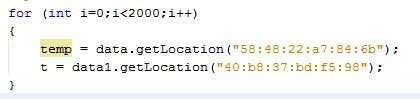
\includegraphics{stream_test.jpg}
		\caption{Stream Test}
		\label{fig:Output}
	\end{figure} 
}
{Critical}
{0}
{Fail}	


